\documentclass{book}
\usepackage[a4paper,top=2.5cm,bottom=2.5cm,left=2.5cm,right=2.5cm]{geometry}
\usepackage{makeidx}
\usepackage{natbib}
\usepackage{graphicx}
\usepackage{multicol}
\usepackage{float}
\usepackage{listings}
\usepackage{color}
\usepackage{ifthen}
\usepackage[table]{xcolor}
\usepackage{textcomp}
\usepackage{alltt}
\usepackage{ifpdf}
\ifpdf
\usepackage[pdftex,
            pagebackref=true,
            colorlinks=true,
            linkcolor=blue,
            unicode
           ]{hyperref}
\else
\usepackage[ps2pdf,
            pagebackref=true,
            colorlinks=true,
            linkcolor=blue,
            unicode
           ]{hyperref}
\usepackage{pspicture}
\fi
\usepackage[utf8]{inputenc}
\usepackage{mathptmx}
\usepackage[scaled=.90]{helvet}
\usepackage{courier}
\usepackage{sectsty}
\usepackage{amssymb}
\usepackage[titles]{tocloft}
\usepackage{doxygen}
\lstset{language=C++,inputencoding=utf8,basicstyle=\footnotesize,breaklines=true,breakatwhitespace=true,tabsize=4,numbers=left }
\makeindex
\setcounter{tocdepth}{3}
\renewcommand{\footrulewidth}{0.4pt}
\renewcommand{\familydefault}{\sfdefault}
\hfuzz=15pt
\setlength{\emergencystretch}{15pt}
\hbadness=750
\tolerance=750
\begin{document}
\hypersetup{pageanchor=false,citecolor=blue}
\begin{titlepage}
\vspace*{7cm}
\begin{center}
{\Large Employee Evaluation \\[1ex]\large 1.\-1 }\\
\vspace*{1cm}
{\large Generated by Doxygen 1.8.3.1}\\
\vspace*{0.5cm}
{\small Sun Jan 27 2013 17:18:59}\\
\end{center}
\end{titlepage}
\clearemptydoublepage
\pagenumbering{roman}
\tableofcontents
\clearemptydoublepage
\pagenumbering{arabic}
\hypersetup{pageanchor=true,citecolor=blue}
\chapter{Hierarchical Index}
\section{Class Hierarchy}
This inheritance list is sorted roughly, but not completely, alphabetically\-:\begin{DoxyCompactList}
\item \contentsline{section}{Entity}{\pageref{class_entity}}{}
\begin{DoxyCompactList}
\item \contentsline{section}{Employee}{\pageref{class_employee}}{}
\item \contentsline{section}{Employer}{\pageref{class_employer}}{}
\end{DoxyCompactList}
\item Q\-Group\-Box\begin{DoxyCompactList}
\item \contentsline{section}{Evaluation}{\pageref{class_evaluation}}{}
\begin{DoxyCompactList}
\item \contentsline{section}{General\-Evaluation}{\pageref{class_general_evaluation}}{}
\end{DoxyCompactList}
\end{DoxyCompactList}
\item Q\-Main\-Window\begin{DoxyCompactList}
\item \contentsline{section}{Main\-Window}{\pageref{class_main_window}}{}
\end{DoxyCompactList}
\item Q\-Widget\begin{DoxyCompactList}
\item \contentsline{section}{Evaluation\-Win}{\pageref{class_evaluation_win}}{}
\end{DoxyCompactList}
\end{DoxyCompactList}

\chapter{Class Index}
\section{Class List}
Here are the classes, structs, unions and interfaces with brief descriptions\-:\begin{DoxyCompactList}
\item\contentsline{section}{\hyperlink{class_employee}{Employee} }{\pageref{class_employee}}{}
\item\contentsline{section}{\hyperlink{class_employer}{Employer} }{\pageref{class_employer}}{}
\item\contentsline{section}{\hyperlink{class_entity}{Entity} }{\pageref{class_entity}}{}
\item\contentsline{section}{\hyperlink{class_evaluation}{Evaluation} }{\pageref{class_evaluation}}{}
\item\contentsline{section}{\hyperlink{class_evaluation_win}{Evaluation\-Win} }{\pageref{class_evaluation_win}}{}
\item\contentsline{section}{\hyperlink{class_general_evaluation}{General\-Evaluation} }{\pageref{class_general_evaluation}}{}
\item\contentsline{section}{\hyperlink{class_main_window}{Main\-Window} }{\pageref{class_main_window}}{}
\end{DoxyCompactList}

\chapter{File Index}
\section{File List}
Here is a list of all documented files with brief descriptions\-:\begin{DoxyCompactList}
\item\contentsline{section}{C\-:/\-Users/\-Noah/\-Documents/\-Qt Projects/\-Employee\-\_\-evaluator/{\bfseries employee.\-h} }{\pageref{employee_8h}}{}
\item\contentsline{section}{C\-:/\-Users/\-Noah/\-Documents/\-Qt Projects/\-Employee\-\_\-evaluator/{\bfseries employer.\-h} }{\pageref{employer_8h}}{}
\item\contentsline{section}{C\-:/\-Users/\-Noah/\-Documents/\-Qt Projects/\-Employee\-\_\-evaluator/\hyperlink{entity_8cpp}{entity.\-cpp} }{\pageref{entity_8cpp}}{}
\item\contentsline{section}{C\-:/\-Users/\-Noah/\-Documents/\-Qt Projects/\-Employee\-\_\-evaluator/\hyperlink{entity_8h}{entity.\-h} }{\pageref{entity_8h}}{}
\item\contentsline{section}{C\-:/\-Users/\-Noah/\-Documents/\-Qt Projects/\-Employee\-\_\-evaluator/\hyperlink{evaluation_8cpp}{evaluation.\-cpp} }{\pageref{evaluation_8cpp}}{}
\item\contentsline{section}{C\-:/\-Users/\-Noah/\-Documents/\-Qt Projects/\-Employee\-\_\-evaluator/\hyperlink{evaluation_8h}{evaluation.\-h} \\*Base widget for each evaluation category. These are added to a tab display for total evaluation }{\pageref{evaluation_8h}}{}
\item\contentsline{section}{C\-:/\-Users/\-Noah/\-Documents/\-Qt Projects/\-Employee\-\_\-evaluator/\hyperlink{evaluationwin_8cpp}{evaluationwin.\-cpp} }{\pageref{evaluationwin_8cpp}}{}
\item\contentsline{section}{C\-:/\-Users/\-Noah/\-Documents/\-Qt Projects/\-Employee\-\_\-evaluator/\hyperlink{evaluationwin_8h}{evaluationwin.\-h} \\*Holds all employee evaluation information to create a new one for an employee }{\pageref{evaluationwin_8h}}{}
\item\contentsline{section}{C\-:/\-Users/\-Noah/\-Documents/\-Qt Projects/\-Employee\-\_\-evaluator/{\bfseries generalevaluation.\-h} }{\pageref{generalevaluation_8h}}{}
\item\contentsline{section}{C\-:/\-Users/\-Noah/\-Documents/\-Qt Projects/\-Employee\-\_\-evaluator/\hyperlink{main_8cpp}{main.\-cpp} }{\pageref{main_8cpp}}{}
\item\contentsline{section}{C\-:/\-Users/\-Noah/\-Documents/\-Qt Projects/\-Employee\-\_\-evaluator/\hyperlink{mainwindow_8cpp}{mainwindow.\-cpp} }{\pageref{mainwindow_8cpp}}{}
\item\contentsline{section}{C\-:/\-Users/\-Noah/\-Documents/\-Qt Projects/\-Employee\-\_\-evaluator/\hyperlink{mainwindow_8h}{mainwindow.\-h} \\*Contains the main window of the program }{\pageref{mainwindow_8h}}{}
\end{DoxyCompactList}

\chapter{Class Documentation}
\hypertarget{class_employee}{\section{Employee Class Reference}
\label{class_employee}\index{Employee@{Employee}}
}


{\ttfamily \#include $<$employee.\-h$>$}

Inheritance diagram for Employee\-:\begin{figure}[H]
\begin{center}
\leavevmode
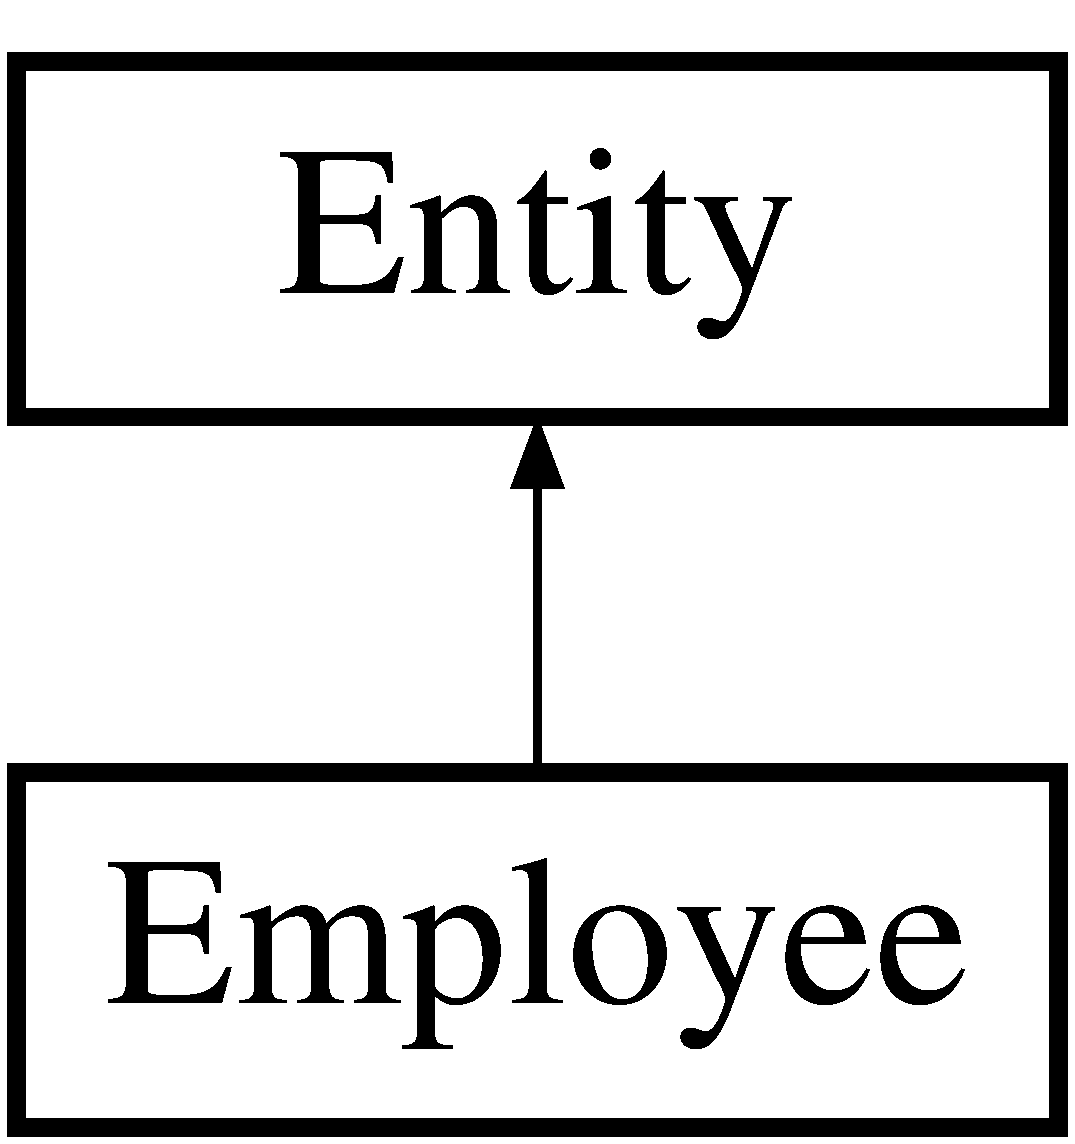
\includegraphics[height=2.000000cm]{class_employee}
\end{center}
\end{figure}
\subsection*{Public Member Functions}
\begin{DoxyCompactItemize}
\item 
\hypertarget{class_employee_a870d18c216c82139c4871ea87c3096a6}{{\bfseries Employee} (int id)}\label{class_employee_a870d18c216c82139c4871ea87c3096a6}

\item 
\hypertarget{class_employee_a67c66a451d22c354f84192450f892f66}{void {\bfseries set\-Name} (Q\-String first, Q\-String last)}\label{class_employee_a67c66a451d22c354f84192450f892f66}

\item 
\hypertarget{class_employee_adb3769cd82ba030068dd96bb6ed4a2e8}{Q\-String {\bfseries get\-First\-Name} ()}\label{class_employee_adb3769cd82ba030068dd96bb6ed4a2e8}

\item 
\hypertarget{class_employee_a129e71f74be20ad0201dedbf62ef31fd}{Q\-String {\bfseries get\-Last\-Name} ()}\label{class_employee_a129e71f74be20ad0201dedbf62ef31fd}

\end{DoxyCompactItemize}
\subsection*{Static Public Member Functions}
\begin{DoxyCompactItemize}
\item 
\hypertarget{class_employee_ae2ba8ebe41c20cfdf75a23b43dea7dfa}{static \hyperlink{class_employee}{Employee} $\ast$ {\bfseries get\-By\-I\-D} (int id)}\label{class_employee_ae2ba8ebe41c20cfdf75a23b43dea7dfa}

\end{DoxyCompactItemize}


\subsection{Detailed Description}
\hyperlink{class_entity}{Entity} with first and last name 

The documentation for this class was generated from the following files\-:\begin{DoxyCompactItemize}
\item 
C\-:/\-Users/\-Noah/\-Documents/\-Qt Projects/\-Employee\-\_\-evaluator/employee.\-h\item 
C\-:/\-Users/\-Noah/\-Documents/\-Qt Projects/\-Employee\-\_\-evaluator/employee.\-cpp\end{DoxyCompactItemize}

\hypertarget{class_employer}{\section{Employer Class Reference}
\label{class_employer}\index{Employer@{Employer}}
}


{\ttfamily \#include $<$employer.\-h$>$}

Inheritance diagram for Employer\-:\begin{figure}[H]
\begin{center}
\leavevmode
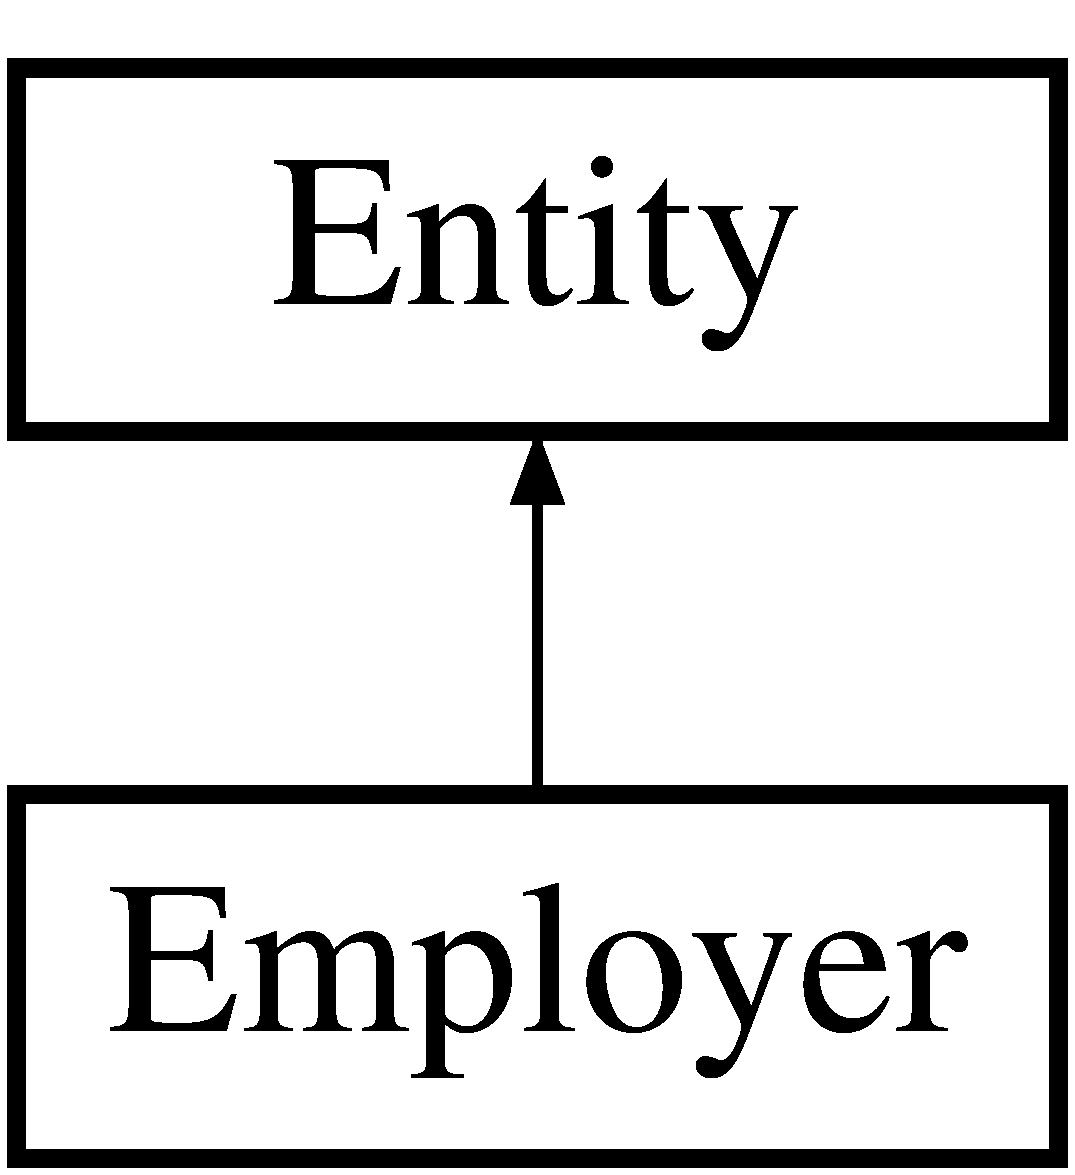
\includegraphics[height=2.000000cm]{class_employer}
\end{center}
\end{figure}
\subsection*{Public Member Functions}
\begin{DoxyCompactItemize}
\item 
\hypertarget{class_employer_a712a6b2e51bd8bd3f02bbac64b2f13a1}{{\bfseries Employer} (int id)}\label{class_employer_a712a6b2e51bd8bd3f02bbac64b2f13a1}

\item 
\hypertarget{class_employer_af9c3bab07b2060255915f986e321cc10}{void {\bfseries set\-Name} (Q\-String name)}\label{class_employer_af9c3bab07b2060255915f986e321cc10}

\item 
\hypertarget{class_employer_aa1608be6c793d947e111dbd474f1de12}{Q\-String {\bfseries get\-Name} ()}\label{class_employer_aa1608be6c793d947e111dbd474f1de12}

\end{DoxyCompactItemize}
\subsection*{Static Public Member Functions}
\begin{DoxyCompactItemize}
\item 
\hypertarget{class_employer_ac9989d539eb2f8489476c90b9ed262cb}{static \hyperlink{class_employer}{Employer} $\ast$ {\bfseries get\-By\-I\-D} (int id)}\label{class_employer_ac9989d539eb2f8489476c90b9ed262cb}

\end{DoxyCompactItemize}


\subsection{Detailed Description}
\hyperlink{class_entity}{Entity} with one company name 

The documentation for this class was generated from the following files\-:\begin{DoxyCompactItemize}
\item 
C\-:/\-Users/\-Noah/\-Documents/\-Qt Projects/\-Employee\-\_\-evaluator/employer.\-h\item 
C\-:/\-Users/\-Noah/\-Documents/\-Qt Projects/\-Employee\-\_\-evaluator/employer.\-cpp\end{DoxyCompactItemize}

\hypertarget{class_entity}{\section{Entity Class Reference}
\label{class_entity}\index{Entity@{Entity}}
}
Inheritance diagram for Entity\-:\begin{figure}[H]
\begin{center}
\leavevmode
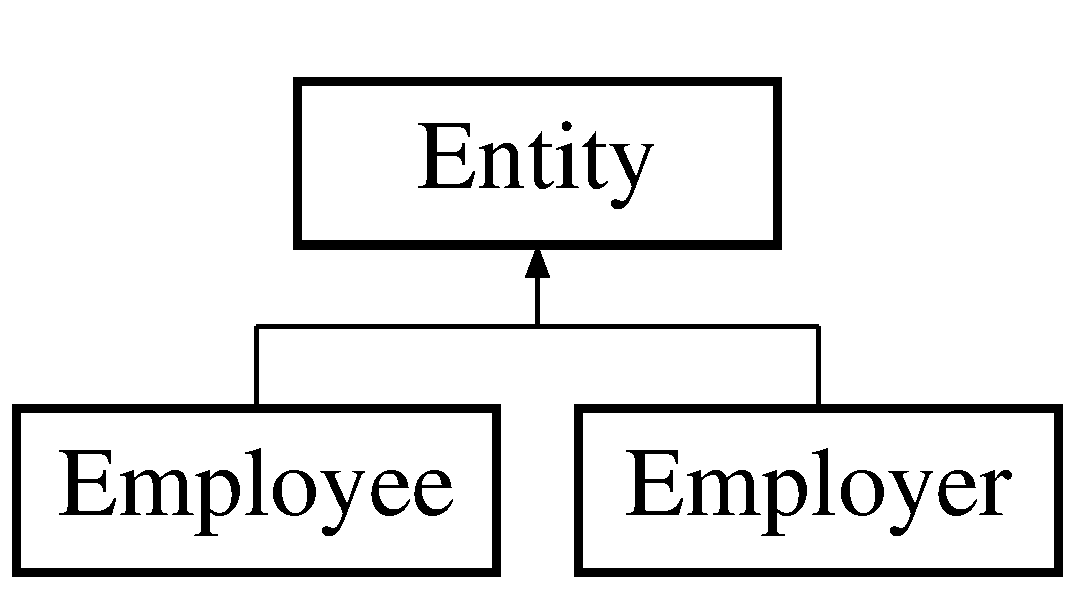
\includegraphics[height=2.000000cm]{class_entity}
\end{center}
\end{figure}
\subsection*{Public Member Functions}
\begin{DoxyCompactItemize}
\item 
\hyperlink{class_entity_a980f368aa07ce358583982821533a54a}{Entity} ()
\item 
\hyperlink{class_entity_ac98bd610e0299cc2aa0538fb2884ab69}{Entity} (int id)
\item 
void \hyperlink{class_entity_a342c3b5da7ceb6c9d983dc8b383f840c}{set\-I\-D} (int id)
\item 
void \hyperlink{class_entity_a8fc9bd93089975942bc43fcb6348b54e}{set\-Email\-Address} (Q\-String email)
\item 
void \hyperlink{class_entity_ae77a743451076f70f2da3376678a9e01}{set\-Phone\-Number} (Q\-String number)
\end{DoxyCompactItemize}
\begin{Indent}{\bf set\-Location}\par
{\em Collectively sets all location info (reduces unneccessary getters/setters) 
\begin{DoxyParams}{Parameters}
{\em address} & The address of the entity. \\
\hline
{\em c} & The city name. \\
\hline
{\em s} & The state name. \\
\hline
{\em zip} & Zip code of the address. \\
\hline
\end{DoxyParams}
}\begin{DoxyCompactItemize}
\item 
\hypertarget{class_entity_a69f8036823da0a5e6b0e7adbc654c815}{void {\bfseries set\-Location} (Q\-String address, Q\-String c, Q\-String s, Q\-String zip)}\label{class_entity_a69f8036823da0a5e6b0e7adbc654c815}

\item 
int \hyperlink{class_entity_a3c60d3c0561843490e93bde1f4566900}{get\-I\-D} ()
\item 
Q\-String \hyperlink{class_entity_a5942a94eb9f88d9c252140a510c38be6}{get\-Email\-Address} ()
\item 
Q\-String \hyperlink{class_entity_a8b9553956f736b82983b5b54a93506ca}{get\-Phone\-Number} ()
\item 
Q\-String \hyperlink{class_entity_a95dfbef7d4957b91d96cc66cc9fc546b}{get\-Street\-Address} ()
\item 
Q\-String \hyperlink{class_entity_a6af4eb490a1be6bf77515d672dc1308f}{get\-City} ()
\item 
Q\-String \hyperlink{class_entity_a6aae5fd0e2271b3321f64529e40977a6}{get\-State} ()
\item 
Q\-String \hyperlink{class_entity_a822e66727444c2f7ef3aee12f0824db8}{get\-Zip\-Code} ()
\end{DoxyCompactItemize}
\end{Indent}


\subsection{Constructor \& Destructor Documentation}
\hypertarget{class_entity_a980f368aa07ce358583982821533a54a}{\index{Entity@{Entity}!Entity@{Entity}}
\index{Entity@{Entity}!Entity@{Entity}}
\subsubsection[{Entity}]{\setlength{\rightskip}{0pt plus 5cm}Entity\-::\-Entity (
\begin{DoxyParamCaption}
{}
\end{DoxyParamCaption}
)}}\label{class_entity_a980f368aa07ce358583982821533a54a}
Default Constructor. Does nothing. \hypertarget{class_entity_ac98bd610e0299cc2aa0538fb2884ab69}{\index{Entity@{Entity}!Entity@{Entity}}
\index{Entity@{Entity}!Entity@{Entity}}
\subsubsection[{Entity}]{\setlength{\rightskip}{0pt plus 5cm}Entity\-::\-Entity (
\begin{DoxyParamCaption}
\item[{int}]{id}
\end{DoxyParamCaption}
)}}\label{class_entity_ac98bd610e0299cc2aa0538fb2884ab69}
Constructor with instantiation of I\-D. 
\begin{DoxyParams}{Parameters}
{\em id} & Unique I\-D of entity. \\
\hline
\end{DoxyParams}


\subsection{Member Function Documentation}
\hypertarget{class_entity_a6af4eb490a1be6bf77515d672dc1308f}{\index{Entity@{Entity}!get\-City@{get\-City}}
\index{get\-City@{get\-City}!Entity@{Entity}}
\subsubsection[{get\-City}]{\setlength{\rightskip}{0pt plus 5cm}Q\-String Entity\-::get\-City (
\begin{DoxyParamCaption}
{}
\end{DoxyParamCaption}
)}}\label{class_entity_a6af4eb490a1be6bf77515d672dc1308f}
\begin{DoxyReturn}{Returns}
City. 
\end{DoxyReturn}
\hypertarget{class_entity_a5942a94eb9f88d9c252140a510c38be6}{\index{Entity@{Entity}!get\-Email\-Address@{get\-Email\-Address}}
\index{get\-Email\-Address@{get\-Email\-Address}!Entity@{Entity}}
\subsubsection[{get\-Email\-Address}]{\setlength{\rightskip}{0pt plus 5cm}Q\-String Entity\-::get\-Email\-Address (
\begin{DoxyParamCaption}
{}
\end{DoxyParamCaption}
)}}\label{class_entity_a5942a94eb9f88d9c252140a510c38be6}
\begin{DoxyReturn}{Returns}
Email address. 
\end{DoxyReturn}
\hypertarget{class_entity_a3c60d3c0561843490e93bde1f4566900}{\index{Entity@{Entity}!get\-I\-D@{get\-I\-D}}
\index{get\-I\-D@{get\-I\-D}!Entity@{Entity}}
\subsubsection[{get\-I\-D}]{\setlength{\rightskip}{0pt plus 5cm}int Entity\-::get\-I\-D (
\begin{DoxyParamCaption}
{}
\end{DoxyParamCaption}
)}}\label{class_entity_a3c60d3c0561843490e93bde1f4566900}
\begin{DoxyReturn}{Returns}
\hyperlink{class_entity}{Entity}'s I\-D. 
\end{DoxyReturn}
\hypertarget{class_entity_a8b9553956f736b82983b5b54a93506ca}{\index{Entity@{Entity}!get\-Phone\-Number@{get\-Phone\-Number}}
\index{get\-Phone\-Number@{get\-Phone\-Number}!Entity@{Entity}}
\subsubsection[{get\-Phone\-Number}]{\setlength{\rightskip}{0pt plus 5cm}Q\-String Entity\-::get\-Phone\-Number (
\begin{DoxyParamCaption}
{}
\end{DoxyParamCaption}
)}}\label{class_entity_a8b9553956f736b82983b5b54a93506ca}
\begin{DoxyReturn}{Returns}
Phone number. 
\end{DoxyReturn}
\hypertarget{class_entity_a6aae5fd0e2271b3321f64529e40977a6}{\index{Entity@{Entity}!get\-State@{get\-State}}
\index{get\-State@{get\-State}!Entity@{Entity}}
\subsubsection[{get\-State}]{\setlength{\rightskip}{0pt plus 5cm}Q\-String Entity\-::get\-State (
\begin{DoxyParamCaption}
{}
\end{DoxyParamCaption}
)}}\label{class_entity_a6aae5fd0e2271b3321f64529e40977a6}
\begin{DoxyReturn}{Returns}
State. 
\end{DoxyReturn}
\hypertarget{class_entity_a95dfbef7d4957b91d96cc66cc9fc546b}{\index{Entity@{Entity}!get\-Street\-Address@{get\-Street\-Address}}
\index{get\-Street\-Address@{get\-Street\-Address}!Entity@{Entity}}
\subsubsection[{get\-Street\-Address}]{\setlength{\rightskip}{0pt plus 5cm}Q\-String Entity\-::get\-Street\-Address (
\begin{DoxyParamCaption}
{}
\end{DoxyParamCaption}
)}}\label{class_entity_a95dfbef7d4957b91d96cc66cc9fc546b}
\begin{DoxyReturn}{Returns}
Street address. 
\end{DoxyReturn}
\hypertarget{class_entity_a822e66727444c2f7ef3aee12f0824db8}{\index{Entity@{Entity}!get\-Zip\-Code@{get\-Zip\-Code}}
\index{get\-Zip\-Code@{get\-Zip\-Code}!Entity@{Entity}}
\subsubsection[{get\-Zip\-Code}]{\setlength{\rightskip}{0pt plus 5cm}Q\-String Entity\-::get\-Zip\-Code (
\begin{DoxyParamCaption}
{}
\end{DoxyParamCaption}
)}}\label{class_entity_a822e66727444c2f7ef3aee12f0824db8}
\begin{DoxyReturn}{Returns}
Zip code. 
\end{DoxyReturn}
\hypertarget{class_entity_a8fc9bd93089975942bc43fcb6348b54e}{\index{Entity@{Entity}!set\-Email\-Address@{set\-Email\-Address}}
\index{set\-Email\-Address@{set\-Email\-Address}!Entity@{Entity}}
\subsubsection[{set\-Email\-Address}]{\setlength{\rightskip}{0pt plus 5cm}void Entity\-::set\-Email\-Address (
\begin{DoxyParamCaption}
\item[{Q\-String}]{email}
\end{DoxyParamCaption}
)}}\label{class_entity_a8fc9bd93089975942bc43fcb6348b54e}
Sets the email addresss of the entity. \hypertarget{class_entity_a342c3b5da7ceb6c9d983dc8b383f840c}{\index{Entity@{Entity}!set\-I\-D@{set\-I\-D}}
\index{set\-I\-D@{set\-I\-D}!Entity@{Entity}}
\subsubsection[{set\-I\-D}]{\setlength{\rightskip}{0pt plus 5cm}void Entity\-::set\-I\-D (
\begin{DoxyParamCaption}
\item[{int}]{id}
\end{DoxyParamCaption}
)}}\label{class_entity_a342c3b5da7ceb6c9d983dc8b383f840c}
Sets the entity's I\-D. \hypertarget{class_entity_ae77a743451076f70f2da3376678a9e01}{\index{Entity@{Entity}!set\-Phone\-Number@{set\-Phone\-Number}}
\index{set\-Phone\-Number@{set\-Phone\-Number}!Entity@{Entity}}
\subsubsection[{set\-Phone\-Number}]{\setlength{\rightskip}{0pt plus 5cm}void Entity\-::set\-Phone\-Number (
\begin{DoxyParamCaption}
\item[{Q\-String}]{number}
\end{DoxyParamCaption}
)}}\label{class_entity_ae77a743451076f70f2da3376678a9e01}
Sets the phone number of the entity. 

The documentation for this class was generated from the following files\-:\begin{DoxyCompactItemize}
\item 
C\-:/\-Users/\-Noah/\-Documents/\-Qt Projects/\-Employee\-\_\-evaluator/\hyperlink{entity_8h}{entity.\-h}\item 
C\-:/\-Users/\-Noah/\-Documents/\-Qt Projects/\-Employee\-\_\-evaluator/\hyperlink{entity_8cpp}{entity.\-cpp}\end{DoxyCompactItemize}

\hypertarget{class_evaluation}{\section{Evaluation Class Reference}
\label{class_evaluation}\index{Evaluation@{Evaluation}}
}
Inheritance diagram for Evaluation\-:\begin{figure}[H]
\begin{center}
\leavevmode
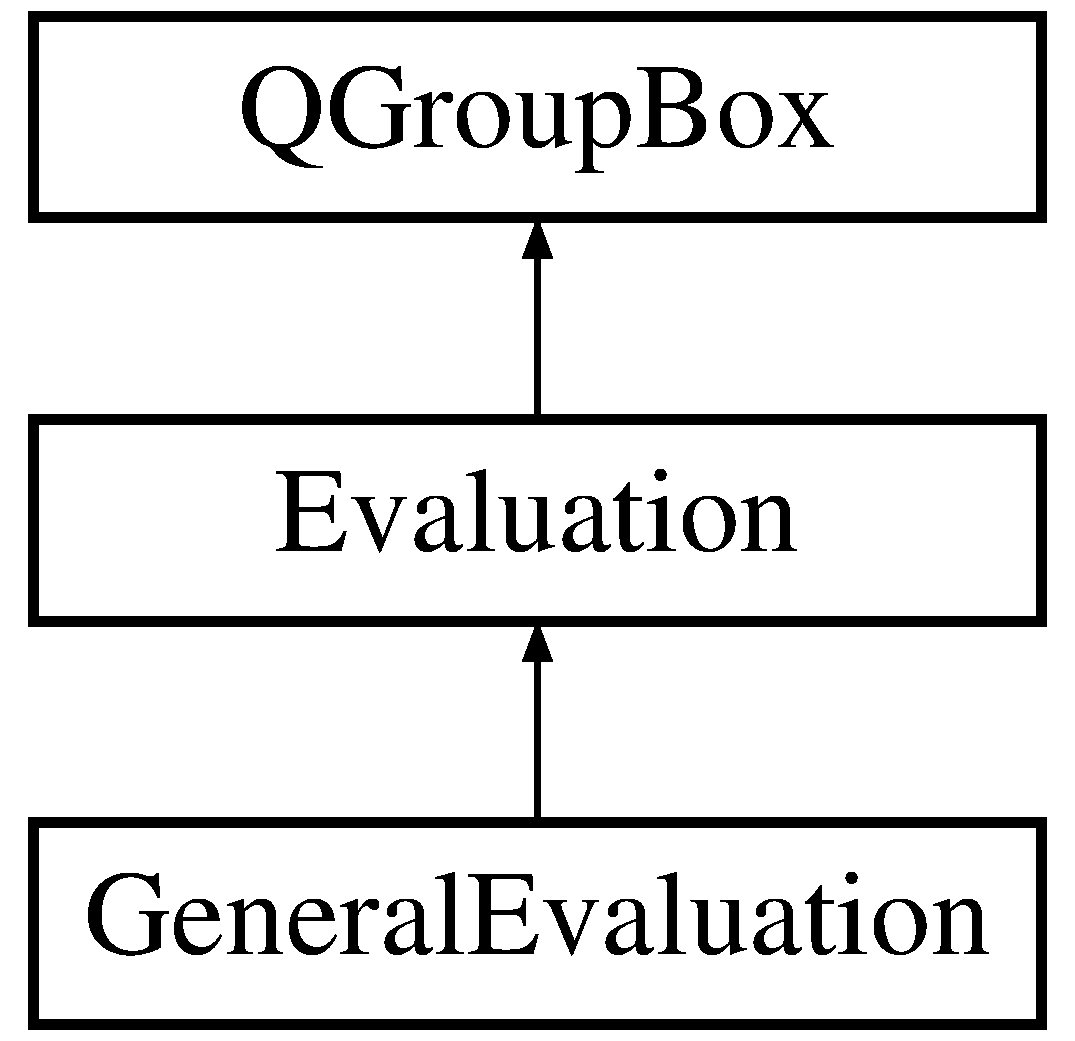
\includegraphics[height=3.000000cm]{class_evaluation}
\end{center}
\end{figure}
\subsection*{Public Slots}
\begin{DoxyCompactItemize}
\item 
void \hyperlink{class_evaluation_affda67750e1fe39d0a066d8850d82abe}{update\-Scale\-Label} ()
\item 
void \hyperlink{class_evaluation_ab2bb3e38d27fa614a094801fa2c656bb}{update\-Char\-Count} ()
\end{DoxyCompactItemize}
\subsection*{Public Member Functions}
\begin{DoxyCompactItemize}
\item 
\hyperlink{class_evaluation_a637c363512d52b26eb5e8ad09d19ff39}{Evaluation} (Q\-String name)
\item 
Q\-String \hyperlink{class_evaluation_a4fbd59ac8bf621c52367fea1f2ff2d3e}{get\-Formatted\-Key} (int val)
\end{DoxyCompactItemize}
\subsection*{Protected Attributes}
\begin{DoxyCompactItemize}
\item 
\hypertarget{class_evaluation_a591ee0e752f624f4dae91882bc57d7c2}{Q\-Label $\ast$ {\bfseries scale\-Label}}\label{class_evaluation_a591ee0e752f624f4dae91882bc57d7c2}

\item 
\hypertarget{class_evaluation_aab8ddd8a9f4fd269d550316833286ec3}{Q\-Label $\ast$ {\bfseries comment\-Label}}\label{class_evaluation_aab8ddd8a9f4fd269d550316833286ec3}

\item 
\hypertarget{class_evaluation_a9e8403e8ef73bcf4bca340b7c7a32ffe}{Q\-Label $\ast$ {\bfseries character\-Count}}\label{class_evaluation_a9e8403e8ef73bcf4bca340b7c7a32ffe}

\item 
\hypertarget{class_evaluation_a2c5368c278af415a12be2dc416bc1261}{Q\-Label $\ast$ {\bfseries character\-Count\-Label}}\label{class_evaluation_a2c5368c278af415a12be2dc416bc1261}

\item 
\hypertarget{class_evaluation_a276bdbdd36c197811002d48dda46fcaa}{Q\-Slider $\ast$ {\bfseries slider}}\label{class_evaluation_a276bdbdd36c197811002d48dda46fcaa}

\item 
\hypertarget{class_evaluation_a02b96d6ec1664ad5af6b6263331e2ac4}{Q\-Text\-Edit $\ast$ {\bfseries comment\-Box}}\label{class_evaluation_a02b96d6ec1664ad5af6b6263331e2ac4}

\item 
\hypertarget{class_evaluation_ac468cfc7353933fe9ed14e7307f2c6aa}{int {\bfseries remaining\-Chars}}\label{class_evaluation_ac468cfc7353933fe9ed14e7307f2c6aa}

\item 
\hypertarget{class_evaluation_a24d7ae8c5320d3520954e1b7db73612c}{Q\-Map$<$ int, Q\-String $>$ $\ast$ {\bfseries scale\-Text\-Map}}\label{class_evaluation_a24d7ae8c5320d3520954e1b7db73612c}

\item 
\hypertarget{class_evaluation_a93a2cbf56a193cec187bb71f1c3ccbd8}{Q\-V\-Box\-Layout $\ast$ {\bfseries layout}}\label{class_evaluation_a93a2cbf56a193cec187bb71f1c3ccbd8}

\end{DoxyCompactItemize}


\subsection{Constructor \& Destructor Documentation}
\hypertarget{class_evaluation_a637c363512d52b26eb5e8ad09d19ff39}{\index{Evaluation@{Evaluation}!Evaluation@{Evaluation}}
\index{Evaluation@{Evaluation}!Evaluation@{Evaluation}}
\subsubsection[{Evaluation}]{\setlength{\rightskip}{0pt plus 5cm}Evaluation\-::\-Evaluation (
\begin{DoxyParamCaption}
\item[{Q\-String}]{name}
\end{DoxyParamCaption}
)}}\label{class_evaluation_a637c363512d52b26eb5e8ad09d19ff39}
Default constructor. Sets the name of the widget. 
\begin{DoxyParams}{Parameters}
{\em name} & Name of the new evaluation widget. \\
\hline
\end{DoxyParams}


\subsection{Member Function Documentation}
\hypertarget{class_evaluation_a4fbd59ac8bf621c52367fea1f2ff2d3e}{\index{Evaluation@{Evaluation}!get\-Formatted\-Key@{get\-Formatted\-Key}}
\index{get\-Formatted\-Key@{get\-Formatted\-Key}!Evaluation@{Evaluation}}
\subsubsection[{get\-Formatted\-Key}]{\setlength{\rightskip}{0pt plus 5cm}Q\-String Evaluation\-::get\-Formatted\-Key (
\begin{DoxyParamCaption}
\item[{int}]{val}
\end{DoxyParamCaption}
)}}\label{class_evaluation_a4fbd59ac8bf621c52367fea1f2ff2d3e}
Returns a formatted string to display given the slider value. 
\begin{DoxyParams}{Parameters}
{\em val} & The value to get a map to \\
\hline
\end{DoxyParams}
\begin{DoxyReturn}{Returns}
Formatted string from map of slider values 
\end{DoxyReturn}
\hypertarget{class_evaluation_ab2bb3e38d27fa614a094801fa2c656bb}{\index{Evaluation@{Evaluation}!update\-Char\-Count@{update\-Char\-Count}}
\index{update\-Char\-Count@{update\-Char\-Count}!Evaluation@{Evaluation}}
\subsubsection[{update\-Char\-Count}]{\setlength{\rightskip}{0pt plus 5cm}void Evaluation\-::update\-Char\-Count (
\begin{DoxyParamCaption}
{}
\end{DoxyParamCaption}
)\hspace{0.3cm}{\ttfamily [slot]}}}\label{class_evaluation_ab2bb3e38d27fa614a094801fa2c656bb}
Updates the characters left in the comments box. \hypertarget{class_evaluation_affda67750e1fe39d0a066d8850d82abe}{\index{Evaluation@{Evaluation}!update\-Scale\-Label@{update\-Scale\-Label}}
\index{update\-Scale\-Label@{update\-Scale\-Label}!Evaluation@{Evaluation}}
\subsubsection[{update\-Scale\-Label}]{\setlength{\rightskip}{0pt plus 5cm}void Evaluation\-::update\-Scale\-Label (
\begin{DoxyParamCaption}
{}
\end{DoxyParamCaption}
)\hspace{0.3cm}{\ttfamily [slot]}}}\label{class_evaluation_affda67750e1fe39d0a066d8850d82abe}
Updates the scale label with the appropriate formatted text. Called when the slider is changed. 

The documentation for this class was generated from the following files\-:\begin{DoxyCompactItemize}
\item 
C\-:/\-Users/\-Noah/\-Documents/\-Qt Projects/\-Employee\-\_\-evaluator/\hyperlink{evaluation_8h}{evaluation.\-h}\item 
C\-:/\-Users/\-Noah/\-Documents/\-Qt Projects/\-Employee\-\_\-evaluator/\hyperlink{evaluation_8cpp}{evaluation.\-cpp}\end{DoxyCompactItemize}

\hypertarget{class_evaluation_win}{\section{Evaluation\-Win Class Reference}
\label{class_evaluation_win}\index{Evaluation\-Win@{Evaluation\-Win}}
}
Inheritance diagram for Evaluation\-Win\-:\begin{figure}[H]
\begin{center}
\leavevmode
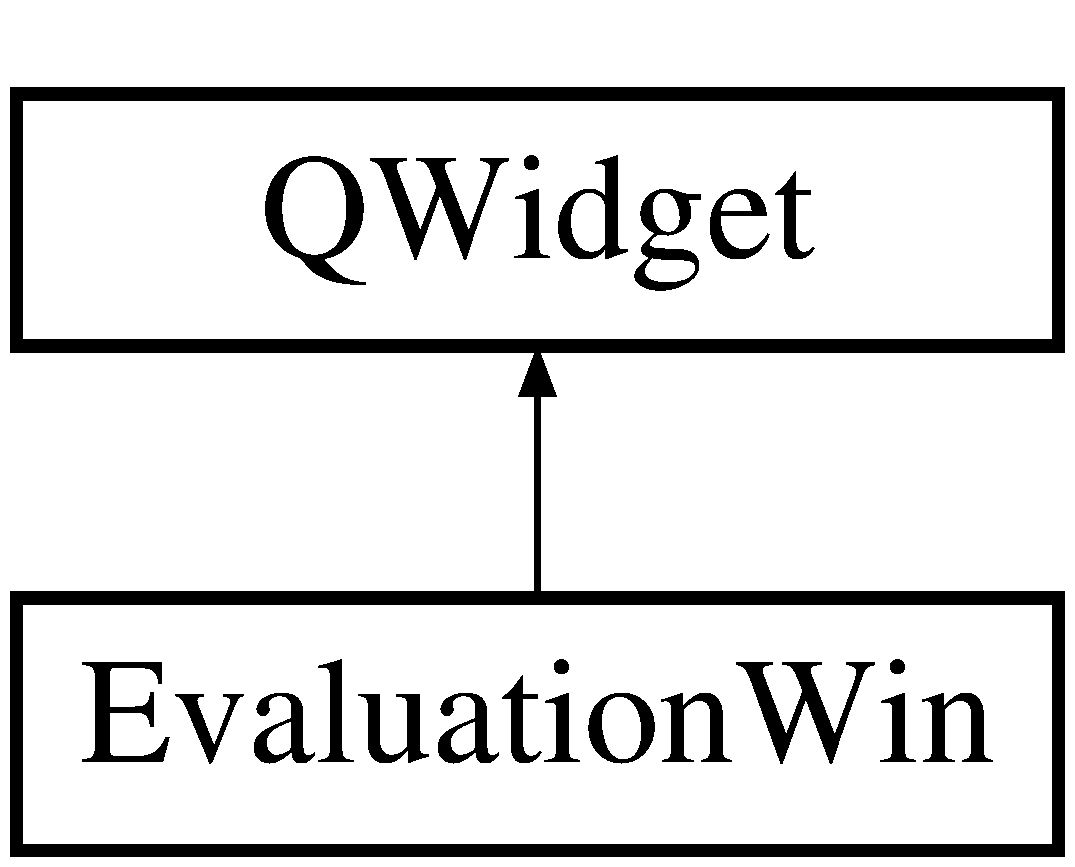
\includegraphics[height=2.000000cm]{class_evaluation_win}
\end{center}
\end{figure}
\subsection*{Public Member Functions}
\begin{DoxyCompactItemize}
\item 
\hypertarget{class_evaluation_win_adc63eca24f260a9bccfb5d3ba28c27d8}{{\bfseries Evaluation\-Win} (Q\-Widget $\ast$parent=0)}\label{class_evaluation_win_adc63eca24f260a9bccfb5d3ba28c27d8}

\end{DoxyCompactItemize}


The documentation for this class was generated from the following files\-:\begin{DoxyCompactItemize}
\item 
C\-:/\-Users/\-Noah/\-Documents/\-Qt Projects/\-Employee\-\_\-evaluator/\hyperlink{evaluationwin_8h}{evaluationwin.\-h}\item 
C\-:/\-Users/\-Noah/\-Documents/\-Qt Projects/\-Employee\-\_\-evaluator/\hyperlink{evaluationwin_8cpp}{evaluationwin.\-cpp}\end{DoxyCompactItemize}

\hypertarget{class_general_evaluation}{\section{General\-Evaluation Class Reference}
\label{class_general_evaluation}\index{General\-Evaluation@{General\-Evaluation}}
}
Inheritance diagram for General\-Evaluation\-:\begin{figure}[H]
\begin{center}
\leavevmode
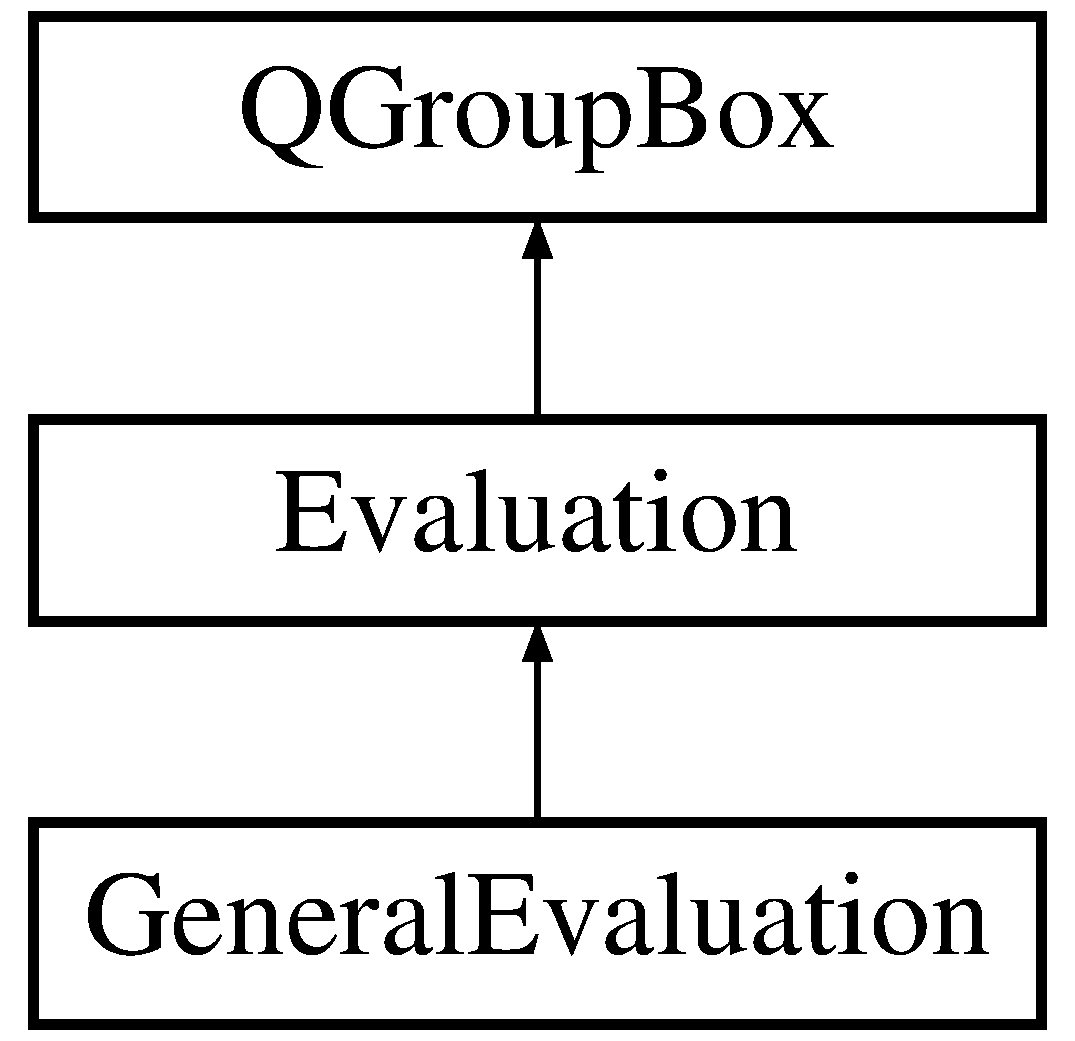
\includegraphics[height=3.000000cm]{class_general_evaluation}
\end{center}
\end{figure}
\subsection*{Public Member Functions}
\begin{DoxyCompactItemize}
\item 
\hyperlink{class_general_evaluation_ac93acb0b867d31acb4070fdcf76c8d94}{General\-Evaluation} (Q\-String name)
\end{DoxyCompactItemize}
\subsection*{Additional Inherited Members}


\subsection{Constructor \& Destructor Documentation}
\hypertarget{class_general_evaluation_ac93acb0b867d31acb4070fdcf76c8d94}{\index{General\-Evaluation@{General\-Evaluation}!General\-Evaluation@{General\-Evaluation}}
\index{General\-Evaluation@{General\-Evaluation}!GeneralEvaluation@{General\-Evaluation}}
\subsubsection[{General\-Evaluation}]{\setlength{\rightskip}{0pt plus 5cm}General\-Evaluation\-::\-General\-Evaluation (
\begin{DoxyParamCaption}
\item[{Q\-String}]{name}
\end{DoxyParamCaption}
)}}\label{class_general_evaluation_ac93acb0b867d31acb4070fdcf76c8d94}
General\-Evaluation.\-cpp 

The documentation for this class was generated from the following files\-:\begin{DoxyCompactItemize}
\item 
C\-:/\-Users/\-Noah/\-Documents/\-Qt Projects/\-Employee\-\_\-evaluator/generalevaluation.\-h\item 
C\-:/\-Users/\-Noah/\-Documents/\-Qt Projects/\-Employee\-\_\-evaluator/generalevaluation.\-cpp\end{DoxyCompactItemize}

\hypertarget{class_main_window}{\section{Main\-Window Class Reference}
\label{class_main_window}\index{Main\-Window@{Main\-Window}}
}
Inheritance diagram for Main\-Window\-:\begin{figure}[H]
\begin{center}
\leavevmode
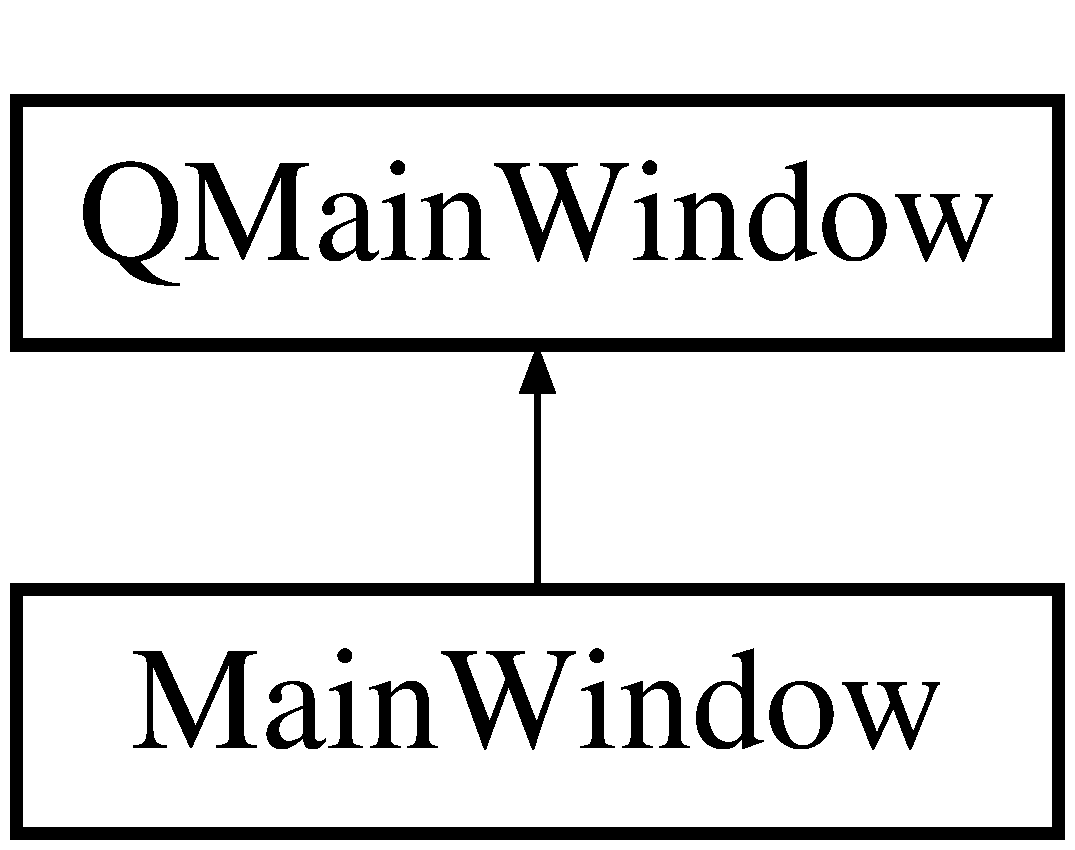
\includegraphics[height=2.000000cm]{class_main_window}
\end{center}
\end{figure}
\subsection*{Public Member Functions}
\begin{DoxyCompactItemize}
\item 
\hypertarget{class_main_window_a34c4b4207b46d11a4100c9b19f0e81bb}{\hyperlink{class_main_window_a34c4b4207b46d11a4100c9b19f0e81bb}{Main\-Window} ()}\label{class_main_window_a34c4b4207b46d11a4100c9b19f0e81bb}

\begin{DoxyCompactList}\small\item\em Default constructor. \end{DoxyCompactList}\end{DoxyCompactItemize}


The documentation for this class was generated from the following files\-:\begin{DoxyCompactItemize}
\item 
C\-:/\-Users/\-Noah/\-Documents/\-Qt Projects/\-Employee\-\_\-evaluator/\hyperlink{mainwindow_8h}{mainwindow.\-h}\item 
C\-:/\-Users/\-Noah/\-Documents/\-Qt Projects/\-Employee\-\_\-evaluator/\hyperlink{mainwindow_8cpp}{mainwindow.\-cpp}\end{DoxyCompactItemize}

\chapter{File Documentation}
\hypertarget{entity_8cpp}{\section{C\-:/\-Users/\-Noah/\-Documents/\-Qt Projects/\-Employee\-\_\-evaluator/entity.cpp File Reference}
\label{entity_8cpp}\index{C\-:/\-Users/\-Noah/\-Documents/\-Qt Projects/\-Employee\-\_\-evaluator/entity.\-cpp@{C\-:/\-Users/\-Noah/\-Documents/\-Qt Projects/\-Employee\-\_\-evaluator/entity.\-cpp}}
}
{\ttfamily \#include \char`\"{}entity.\-h\char`\"{}}\\*
{\ttfamily \#include $<$Q\-String$>$}\\*

\hypertarget{entity_8h}{\section{C\-:/\-Users/\-Noah/\-Documents/\-Qt Projects/\-Employee\-\_\-evaluator/entity.h File Reference}
\label{entity_8h}\index{C\-:/\-Users/\-Noah/\-Documents/\-Qt Projects/\-Employee\-\_\-evaluator/entity.\-h@{C\-:/\-Users/\-Noah/\-Documents/\-Qt Projects/\-Employee\-\_\-evaluator/entity.\-h}}
}
{\ttfamily \#include $<$Q\-String$>$}\\*
\subsection*{Classes}
\begin{DoxyCompactItemize}
\item 
class \hyperlink{class_entity}{Entity}
\end{DoxyCompactItemize}


\subsection{Detailed Description}
Base class for the employer and employee classes. This holds the common properties between the two. 
\hypertarget{evaluation_8cpp}{\section{C\-:/\-Users/\-Noah/\-Documents/\-Qt Projects/\-Employee\-\_\-evaluator/evaluation.cpp File Reference}
\label{evaluation_8cpp}\index{C\-:/\-Users/\-Noah/\-Documents/\-Qt Projects/\-Employee\-\_\-evaluator/evaluation.\-cpp@{C\-:/\-Users/\-Noah/\-Documents/\-Qt Projects/\-Employee\-\_\-evaluator/evaluation.\-cpp}}
}
{\ttfamily \#include \char`\"{}evaluation.\-h\char`\"{}}\\*
{\ttfamily \#include $<$Q\-Slider$>$}\\*
{\ttfamily \#include $<$Q\-Text\-Edit$>$}\\*
{\ttfamily \#include $<$Q\-V\-Box\-Layout$>$}\\*
{\ttfamily \#include $<$Q\-Label$>$}\\*
{\ttfamily \#include $<$Q\-Debug$>$}\\*

\hypertarget{evaluation_8h}{\section{C\-:/\-Users/\-Noah/\-Documents/\-Qt Projects/\-Employee\-\_\-evaluator/evaluation.h File Reference}
\label{evaluation_8h}\index{C\-:/\-Users/\-Noah/\-Documents/\-Qt Projects/\-Employee\-\_\-evaluator/evaluation.\-h@{C\-:/\-Users/\-Noah/\-Documents/\-Qt Projects/\-Employee\-\_\-evaluator/evaluation.\-h}}
}


Base widget for each evaluation category. These are added to a tab display for total evaluation.  


{\ttfamily \#include $<$Q\-Group\-Box$>$}\\*
{\ttfamily \#include $<$Q\-Map$>$}\\*
\subsection*{Classes}
\begin{DoxyCompactItemize}
\item 
class \hyperlink{class_evaluation}{Evaluation}
\end{DoxyCompactItemize}


\subsection{Detailed Description}
Base widget for each evaluation category. These are added to a tab display for total evaluation. 
\hypertarget{evaluationwin_8cpp}{\section{C\-:/\-Users/\-Noah/\-Documents/\-Qt Projects/\-Employee\-\_\-evaluator/evaluationwin.cpp File Reference}
\label{evaluationwin_8cpp}\index{C\-:/\-Users/\-Noah/\-Documents/\-Qt Projects/\-Employee\-\_\-evaluator/evaluationwin.\-cpp@{C\-:/\-Users/\-Noah/\-Documents/\-Qt Projects/\-Employee\-\_\-evaluator/evaluationwin.\-cpp}}
}
{\ttfamily \#include \char`\"{}evaluationwin.\-h\char`\"{}}\\*
{\ttfamily \#include \char`\"{}generalevaluation.\-h\char`\"{}}\\*
{\ttfamily \#include $<$Q\-V\-Box\-Layout$>$}\\*
{\ttfamily \#include $<$Q\-Tab\-Widget$>$}\\*
{\ttfamily \#include $<$Q\-Status\-Bar$>$}\\*
{\ttfamily \#include \char`\"{}evaluation.\-h\char`\"{}}\\*
{\ttfamily \#include $<$Q\-Label$>$}\\*
\subsection*{Variables}
\begin{DoxyCompactItemize}
\item 
\hypertarget{evaluationwin_8cpp_acaf6a0c5380308f4b8787cf141efaf93}{const int {\bfseries win\-X} = 450}\label{evaluationwin_8cpp_acaf6a0c5380308f4b8787cf141efaf93}

\item 
\hypertarget{evaluationwin_8cpp_ac52638d5dd2222785bdbdac28874c73c}{const int {\bfseries win\-Y} = 500}\label{evaluationwin_8cpp_ac52638d5dd2222785bdbdac28874c73c}

\end{DoxyCompactItemize}

\hypertarget{evaluationwin_8h}{\section{C\-:/\-Users/\-Noah/\-Documents/\-Qt Projects/\-Employee\-\_\-evaluator/evaluationwin.h File Reference}
\label{evaluationwin_8h}\index{C\-:/\-Users/\-Noah/\-Documents/\-Qt Projects/\-Employee\-\_\-evaluator/evaluationwin.\-h@{C\-:/\-Users/\-Noah/\-Documents/\-Qt Projects/\-Employee\-\_\-evaluator/evaluationwin.\-h}}
}


Holds all employee evaluation information to create a new one for an employee.  


{\ttfamily \#include $<$Q\-Widget$>$}\\*
\subsection*{Classes}
\begin{DoxyCompactItemize}
\item 
class \hyperlink{class_evaluation_win}{Evaluation\-Win}
\end{DoxyCompactItemize}


\subsection{Detailed Description}
Holds all employee evaluation information to create a new one for an employee. 
\hypertarget{main_8cpp}{\section{C\-:/\-Users/\-Noah/\-Documents/\-Qt Projects/\-Employee\-\_\-evaluator/main.cpp File Reference}
\label{main_8cpp}\index{C\-:/\-Users/\-Noah/\-Documents/\-Qt Projects/\-Employee\-\_\-evaluator/main.\-cpp@{C\-:/\-Users/\-Noah/\-Documents/\-Qt Projects/\-Employee\-\_\-evaluator/main.\-cpp}}
}
{\ttfamily \#include $<$Qt\-Gui/\-Q\-Application$>$}\\*
{\ttfamily \#include \char`\"{}mainwindow.\-h\char`\"{}}\\*
{\ttfamily \#include \char`\"{}employee.\-h\char`\"{}}\\*
{\ttfamily \#include \char`\"{}evaluationwin.\-h\char`\"{}}\\*
\subsection*{Functions}
\begin{DoxyCompactItemize}
\item 
\hypertarget{main_8cpp_a0ddf1224851353fc92bfbff6f499fa97}{int {\bfseries main} (int argc, char $\ast$argv\mbox{[}$\,$\mbox{]})}\label{main_8cpp_a0ddf1224851353fc92bfbff6f499fa97}

\end{DoxyCompactItemize}


\subsection{Detailed Description}
The main class of the program. Launches the main window. 
\hypertarget{mainwindow_8cpp}{\section{C\-:/\-Users/\-Noah/\-Documents/\-Qt Projects/\-Employee\-\_\-evaluator/mainwindow.cpp File Reference}
\label{mainwindow_8cpp}\index{C\-:/\-Users/\-Noah/\-Documents/\-Qt Projects/\-Employee\-\_\-evaluator/mainwindow.\-cpp@{C\-:/\-Users/\-Noah/\-Documents/\-Qt Projects/\-Employee\-\_\-evaluator/mainwindow.\-cpp}}
}
{\ttfamily \#include \char`\"{}mainwindow.\-h\char`\"{}}\\*
{\ttfamily \#include $<$Q\-V\-Box\-Layout$>$}\\*
{\ttfamily \#include $<$Q\-Tab\-Widget$>$}\\*
{\ttfamily \#include $<$Q\-Status\-Bar$>$}\\*
{\ttfamily \#include \char`\"{}evaluation.\-h\char`\"{}}\\*
{\ttfamily \#include $<$Q\-Label$>$}\\*
\subsection*{Variables}
\begin{DoxyCompactItemize}
\item 
\hypertarget{mainwindow_8cpp_acaf6a0c5380308f4b8787cf141efaf93}{const int {\bfseries win\-X} = 450}\label{mainwindow_8cpp_acaf6a0c5380308f4b8787cf141efaf93}

\item 
\hypertarget{mainwindow_8cpp_ac52638d5dd2222785bdbdac28874c73c}{const int {\bfseries win\-Y} = 500}\label{mainwindow_8cpp_ac52638d5dd2222785bdbdac28874c73c}

\item 
\hypertarget{mainwindow_8cpp_ac758281b955228554700009c2ca2bf34}{const int {\bfseries status\-X} = win\-X}\label{mainwindow_8cpp_ac758281b955228554700009c2ca2bf34}

\item 
\hypertarget{mainwindow_8cpp_a2d4740cc0efb80008a3e8b7656d88290}{const int {\bfseries status\-Y} = 50}\label{mainwindow_8cpp_a2d4740cc0efb80008a3e8b7656d88290}

\end{DoxyCompactItemize}

\hypertarget{mainwindow_8h}{\section{C\-:/\-Users/\-Noah/\-Documents/\-Qt Projects/\-Employee\-\_\-evaluator/mainwindow.h File Reference}
\label{mainwindow_8h}\index{C\-:/\-Users/\-Noah/\-Documents/\-Qt Projects/\-Employee\-\_\-evaluator/mainwindow.\-h@{C\-:/\-Users/\-Noah/\-Documents/\-Qt Projects/\-Employee\-\_\-evaluator/mainwindow.\-h}}
}


Contains the main window of the program.  


{\ttfamily \#include $<$Q\-Widget$>$}\\*
{\ttfamily \#include $<$Q\-Main\-Window$>$}\\*
\subsection*{Classes}
\begin{DoxyCompactItemize}
\item 
class \hyperlink{class_main_window}{Main\-Window}
\end{DoxyCompactItemize}


\subsection{Detailed Description}
Contains the main window of the program. 
\addcontentsline{toc}{part}{Index}
\printindex
\end{document}
